\documentclass[11pt]{article}

\usepackage[margin=0.7in]{geometry}
\usepackage{amsmath,amssymb}
\usepackage{tikz}
\usetikzlibrary{arrows.meta,decorations.pathreplacing,positioning}

\pagestyle{empty}

\begin{document}

\begin{figure}[ht]
\centering
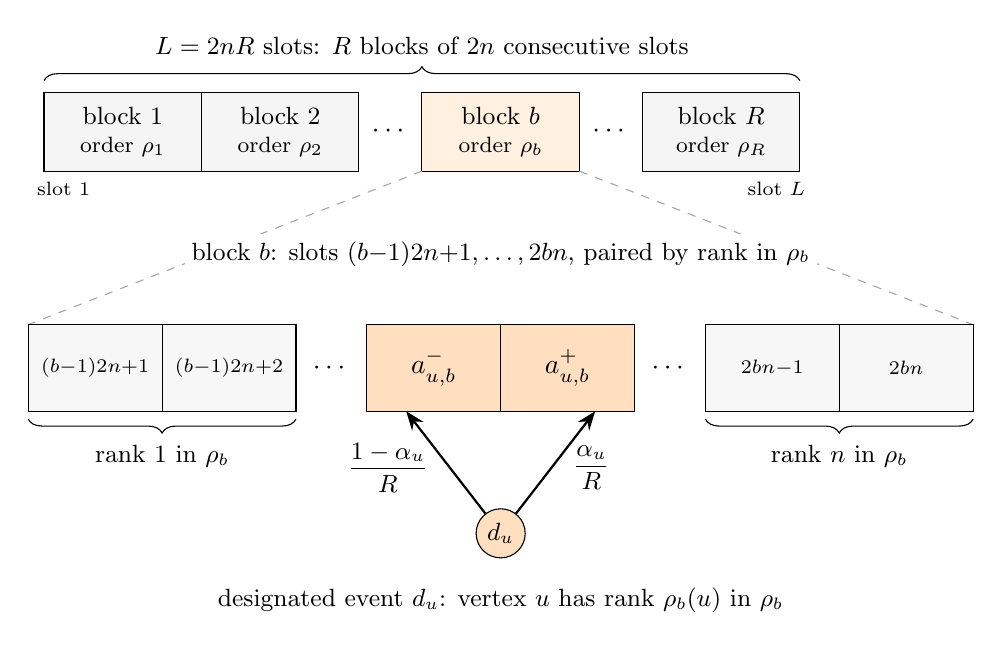
\begin{tikzpicture}[
  blockbox/.style={draw, fill=gray!8, minimum height=10mm, align=center, font=\small},
  slotbox/.style={draw, fill=gray!6, minimum height=11mm, align=center},
  duslot/.style={draw, fill=orange!25, minimum height=11mm, align=center},
  zoom/.style={dashed, gray!70},
  brace/.style={decorate, decoration={brace, amplitude=5pt}},
  mbrace/.style={decorate, decoration={brace, mirror, amplitude=5pt}},
  dep/.style={-{Stealth[length=2.4mm]}, thick},
  lab/.style={font=\small}
]

% ---------- Top strip: the R blocks ----------
\draw[blockbox] (0.2,4.4) rectangle (2.2,5.4);
\node[align=center, font=\small] at (1.2,4.9) {block $1$\\[-1pt] {\footnotesize order $\rho_1$}};
\draw[blockbox] (2.2,4.4) rectangle (4.2,5.4);
\node[align=center, font=\small] at (3.2,4.9) {block $2$\\[-1pt] {\footnotesize order $\rho_2$}};
\node at (4.6,4.9) {$\cdots$};
\draw[fill=orange!12] (5.0,4.4) rectangle (7.0,5.4);
\node[align=center, font=\small] at (6.0,4.9) {block $b$\\[-1pt] {\footnotesize order $\rho_b$}};
\node at (7.4,4.9) {$\cdots$};
\draw[blockbox] (7.8,4.4) rectangle (9.8,5.4);
\node[align=center, font=\small] at (8.8,4.9) {block $R$\\[-1pt] {\footnotesize order $\rho_R$}};

% overall brace
\draw[brace] (0.2,5.55) -- (9.8,5.55)
  node[midway, above=6pt, lab] {$L=2nR$ slots: $R$ blocks of $2n$ consecutive slots};

% end-slot ticks
\node[below, font=\scriptsize] at (0.45,4.38) {slot $1$};
\node[below, font=\scriptsize] at (9.5,4.38) {slot $L$};

% ---------- Zoom lines ----------
\draw[zoom] (5.0,4.4) -- (0,2.45);
\draw[zoom] (7.0,4.4) -- (12,2.45);
\node[font=\small, fill=white, inner sep=2.5pt] at (6.0,3.35)
  {block $b$: slots $(b{-}1)2n{+}1,\ldots,2bn$, paired by rank in $\rho_b$};

% ---------- Detail strip: inside block b ----------
% pair at rank 1
\draw[slotbox] (0,1.35)   rectangle (1.7,2.45);
\node[font=\scriptsize] at (0.85,1.9) {$(b{-}1)2n{+}1$};
\draw[slotbox] (1.7,1.35) rectangle (3.4,2.45);
\node[font=\scriptsize] at (2.55,1.9) {$(b{-}1)2n{+}2$};
\node at (3.85,1.9) {$\cdots$};
% pair at rank rho_b(u): the designated pair of u
\draw[duslot] (4.3,1.35)  rectangle (6.0,2.45);
\node at (5.15,1.9) {$a^-_{u,b}$};
\draw[duslot] (6.0,1.35)  rectangle (7.7,2.45);
\node at (6.85,1.9) {$a^+_{u,b}$};
\node at (8.15,1.9) {$\cdots$};
% pair at rank n
\draw[slotbox] (8.6,1.35)  rectangle (10.3,2.45);
\node[font=\scriptsize] at (9.45,1.9) {$2bn{-}1$};
\draw[slotbox] (10.3,1.35) rectangle (12,2.45);
\node[font=\scriptsize] at (11.15,1.9) {$2bn$};

% rank braces for the outer pairs
\draw[mbrace] (0,1.25) -- (3.4,1.25)
  node[midway, below=6pt, font=\small] {rank $1$ in $\rho_b$};
\draw[mbrace] (8.6,1.25) -- (12,1.25)
  node[midway, below=6pt, font=\small] {rank $n$ in $\rho_b$};

% designated event d_u and its two slots
\node[draw, circle, fill=orange!25, inner sep=2pt, font=\small] (du) at (6.0,-0.2) {$d_u$};
\draw[dep] (du) -- (4.8,1.35)
  node[pos=0.45, left=4pt, font=\small] {$\dfrac{1-\alpha_u}{R}$};
\draw[dep] (du) -- (7.2,1.35)
  node[pos=0.45, right=4pt, font=\small] {$\dfrac{\alpha_u}{R}$};
\node[font=\small, align=center] at (6.0,-1.05)
  {designated event $d_u$: vertex $u$ has rank $\rho_b(u)$ in $\rho_b$};

\end{tikzpicture}

\caption{Slot layout of the constructed ORP instance.  The $L=2nR$ slots are
partitioned into $R$ consecutive blocks of width $2n$, and block $b$ is
associated with the profile order $\rho_b$.  Within block $b$, the vertex of
rank $r$ in $\rho_b$ owns the consecutive slot pair
$\bigl((b{-}1)2n+2r-1,\;(b{-}1)2n+2r\bigr)$; for vertex $u$ this is the pair
$a^-_{u,b}=(b{-}1)2n+2\rho_b(u)-1$ and $a^+_{u,b}=(b{-}1)2n+2\rho_b(u)$.
Given the observation vector $\hat t=0$, the designated event $d_u$ occupies
slot $a^-_{u,b}$ with probability $(1-\alpha_u)/R$ and slot $a^+_{u,b}$ with
probability $\alpha_u/R$, for each block $b\in\{1,\ldots,R\}$ (Lemma~4,
Independence via fillers), where
$\alpha_u=\tfrac12-\tfrac{2\delta_u}{R}+\tfrac{\delta_u}{R^2}$.  Each of the
$q=L-n$ filler events has uniform noise, with mass $1/L$ on $-s$ for
$s=1,\ldots,L$.}
\end{figure}

\end{document}
